\documentclass[11pt]{article}

\usepackage{amsmath}
\usepackage{amssymb}
\usepackage[margin=1in]{geometry}
\usepackage{microtype}
\usepackage{siunitx}
\usepackage{graphicx}
\usepackage{hyperref}

% --- Convenience macros ---
\newcommand{\dtype}[1]{\mathrm{#1}}          % data-type names: \dtype{int8}, \dtype{bf16}
\newcommand{\contract}[1]{\cdot_{#1}}         % contraction over an index: A \contract{D} B
\newcommand{\Tmath}{T_{\text{math}}}
\newcommand{\Tcomms}{T_{\text{comms}}}
\newcommand{\Icrit}{I_{\text{crit}}}

\sisetup{
  exponent-product = \times,
  per-mode         = symbol,
}

\title{How to Scale Your Model: Part 1 Roofline Exercises}
\author{Asher Tooley}
\date{}

\begin{document}

\maketitle

\section{\texorpdfstring{\(\dtype{int8}\)}{int8} Matmul}

We consider the operation
\[
\dtype{int8}[B,D]\contract{D}\dtype{int8}[D,F]
\;\to\;
\dtype{int8}[B,F],
\]
where \(A \contract{D} B\) denotes contraction (matrix multiplication) over the
shared index \(D\). An \(\dtype{int8}\) value occupies \qty{1}{byte} and a
\(\dtype{bf16}\) value occupies \qty{2}{bytes}; all calculations assume each
tensor is read from HBM once and the output written back once.

Since \(\dtype{int8}\) uses \qty{1}{byte} per value, the bytes loaded are
\(BD + DF\) and the bytes written back are \(BF\), giving total memory traffic
\(BD + DF + BF\). There are \(BF\) output entries, each a dot product over \(D\)
requiring \(D\) multiplications and \(D-1\) additions, so the exact operation
count is \(BF(2D-1)\approx 2BDF\). The arithmetic intensity is therefore
\begin{align}
I
&= \frac{2BDF}{BD+DF+BF}
   \approx \frac{2BDF}{DF}
   = 2B,
\end{align}
where the approximation assumes \(B\) is small relative to \(D\) and \(F\), so the
\(DF\) term dominates the denominator. The critical arithmetic intensity is
\begin{align}
\Icrit
&= \frac{\num{3.94e14}}{\num{8.2e11}}
   \approx 480,
\end{align}
so the operation becomes compute-bound when \(2B \gtrsim 480\), i.e.
\(B \gtrsim 240\). The runtime bounds follow from
\begin{align}
\Tmath  &= \frac{2BDF}{\num{3.94e14}}, &
\Tcomms &= \frac{BD+DF+BF}{\num{8.2e11}},
\end{align}
with a reasonable lower bound \(T_{\text{lower}} = \max(\Tmath, \Tcomms)\) and
upper bound \(T_{\text{upper}} = \Tmath + \Tcomms\).

\section{\texorpdfstring{\(\dtype{int8}\)}{int8} Weights and \texorpdfstring{\(\dtype{bf16}\)}{bf16} Activations}

We consider the operation
\[
\dtype{bf16}[B,D]\contract{D}\dtype{int8}[D,F]
\;\to\;
\dtype{bf16}[B,F].
\]

The operation count is still \(\approx 2BDF\). The \(\dtype{bf16}\) activations
cost \(2BD\) bytes to load, the \(\dtype{int8}\) weights cost \(DF\) bytes, and the
\(\dtype{bf16}\) output costs \(2BF\) bytes, for total traffic
\(2BD + DF + 2BF\). Hence
\begin{align}
I
&= \frac{2BDF}{2BD+DF+2BF}
   \approx \frac{2BDF}{DF}
   = 2B.
\end{align}
The critical arithmetic intensity for \(\dtype{bf16}\) compute is
\begin{align}
\Icrit
&= \frac{\num{1.97e14}}{\num{8.2e11}}
   \approx 240,
\end{align}
so the operation becomes compute-bound when \(2B \gtrsim 240\), i.e.
\(B \gtrsim 120\).

\section{Roofline Plot}

The roofline plot uses the exact memory traffic from Section~2,
\(2BD + DF + 2BF\), rather than the large-\(D,F\) approximation. For each \(B\),
the achieved throughput is
\[
\text{Achieved FLOPs/s}
= \frac{2BDF}{\max(\Tmath,\Tcomms)},
\]
where
\begin{align}
\Tmath  &= \frac{2BDF}{\num{1.97e14}}, &
\Tcomms &= \frac{2BD+DF+2BF}{\num{8.2e11}}.
\end{align}
The two plotted cases are \(D=F=4096\) and \(D=F=1024\).

\begin{figure}[ht]
  \centering
  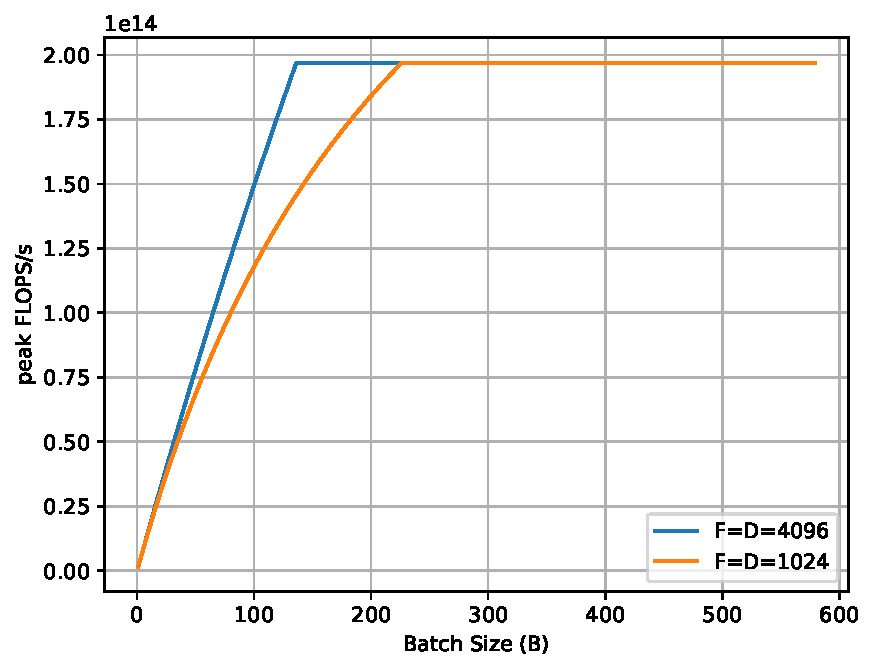
\includegraphics[width=0.75\textwidth]{roofline_fig.pdf}
  \caption{Achieved throughput versus batch size for \(D=F=4096\) and
  \(D=F=1024\).}
  \label{fig:roofline}
\end{figure}

\clearpage
\section{Per-Batch \texorpdfstring{\(\dtype{int8}\)}{int8} Matrices}

We consider the operation
\[
\dtype{int8}[B,D]\contract{D}\dtype{int8}[B,D,F]
\;\to\;
\dtype{int8}[B,F].
\]

There are still \(BF\) output entries, each a dot product over \(D\), so the
operation count is \(\approx 2BDF\). Memory traffic is larger because each batch
element carries its own \(D\times F\) matrix: loading the first input costs
\(BD\) bytes, the second costs \(BDF\) bytes, and the output costs \(BF\) bytes,
for total traffic \(BD + BDF + BF\). Therefore
\begin{align}
I
&= \frac{2BDF}{BD+BDF+BF}
   = \frac{2DF}{D+DF+F}
   \approx \frac{2DF}{DF}
   = 2,
\end{align}
where factoring out \(B\) shows the intensity is independent of batch size, and
the \(DF\) term dominates for large \(D,F\). Unlike ordinary matrix
multiplication, increasing the batch size does not improve arithmetic intensity,
because each batch element has its own matrix. This operation is therefore
generally memory-bandwidth bound.

\section{H100 SXM \texorpdfstring{\(\dtype{bf16}\)}{bf16} Matmul}

For the H100 SXM, the reported \(\dtype{bf16}\) Tensor Core performance is
\num{1.979e15}~FLOPs/s, but this figure assumes structured sparsity. The dense
\(\dtype{bf16}\) value is half of this:
\[
\frac{\num{1.979e15}}{2} = \num{9.89e14}~\text{FLOPs/s}.
\]
With HBM bandwidth \qty{3.35}{TB/s} \(=\) \num{3.35e12}~bytes/s, the critical
arithmetic intensity is
\begin{align}
\Icrit
&= \frac{\num{9.89e14}}{\num{3.35e12}}
   \approx 295.
\end{align}
For a standard \(\dtype{bf16}\) matmul the arithmetic intensity is
\(I \approx B\), so the operation becomes compute-bound when \(B \gtrsim 295\).

\end{document}